\documentclass[article,11pt, a4paper,sumario=tradicional]{abntex2}
\usepackage{lmodern}                    % Usa a fonte Latin Modern
\usepackage[T1]{fontenc}                % Selecao de codigos de fonte.
\usepackage[utf8]{inputenc}             % Codificacao do documento (conversão automática dos acentos)
\usepackage{indentfirst}                % Indenta o primeiro parágrafo de cada seção.
\usepackage{nomencl}                    % Lista de simbolos
\usepackage{color}                              % Controle das cores
\usepackage{graphicx}                   % Inclusão de gráficos
\usepackage{microtype}                  % para melhorias de justificação

% ---
% Altera as margens padrões
% ---
\setlrmarginsandblock{3cm}{3cm}{*}
\setulmarginsandblock{3cm}{3cm}{*}
\checkandfixthelayout
% ---

% --- 
% Espaçamentos entre linhas e parágrafos 
% --- 

% O tamanho do parágrafo é dado por:
\setlength{\parindent}{1.3cm}

% Controle do espaçamento entre um parágrafo e outro:
\setlength{\parskip}{0.2cm}  % tente também \onelineskip

% Espaçamento simples
\SingleSpacing

% alterando o aspecto da cor azul
\definecolor{blue}{RGB}{41,5,195}
% para o pdf
\makeatletter
\hypersetup{
 linkcolor=blue,                 % color of internal links
 citecolor=blue,                 % color of links to bibliography
 filecolor=magenta,              % color of file links
 urlcolor=blue,
}

%opening
\titulo{Abordando o jogo 0A.D. em sala de aula}
\autor{Lincoln de Macêdo \\ Renan Tomazini}

\begin{document}

\maketitle

\textual

\begin{abstract}
    Este é um simples resumo de perspectivas sobre a abordagem de um jogo RTS (\textit{Real Time Strategy}) com foco na ciência histórica tomando como exemplo o jogo 0A.D. Trazendo luz também a pontos chave que possam servir ao desenvolvimento de jogos educacionais com foco e jogabilidade semelhantes.
\end{abstract}

\section{Características e definições}
    Como o nome já indica, um jogo de estratégia em tempo real visa proporcionar o dinamismo da ação com a perspectiva e raciocínio exigidos em jogos de clássicos de estratégia. O grande diferencial aqui está no acompanhamento, recursos e respostas feitas a partir de cada movimentação, podemos dividir de modo geral uma partida em dois momentos: 1 -- administração de recursos e 2 -- estratégia de combate. Ainda em termos gerais iniciamos uma partida com recursos mínimos e temos a tarefa de fazer a economia prosperar e com isso ter condições de aumentar a população com o intuíto de expandir o território e consequentemente conquistar territórios vizinhos.

    No jogo 0A.D. escolhemos um dos povos da antiguidade clássica\footnote{Ao fim do documento há mais detalhes sobre os povos retratados no jogo}, inserido num determinado bioma, numa determinada geografia, agindo como um posto avançado ou colônia e tendo de interagir pacificamente ou belicamente com seu(s) vizinho(s) e ainda havendo a possibilidade de reproduzir batalhas históricas, temos os passos básicos de evolução da partida descritos no parágrafo anterior com alguns acrécimos relativos ao nível de desenvolvimento social, cultural e tecnológico do povo escolhido (elementos que ainda podem variar dependendo da localização geográfica em que se iniciou a partida).

    A imersão, característica tão fundamental nos jogos digitais, se dá ao longo da fase administrativa já que é aí que se conhece algumas características culturais e como o jogador se coloca como o líder do povo escolhido, a identificação ocorre naturalnente. Estes pontos levam o jogador a atingir o que é esperado num jogo digital: uma experiência completa ao nível sensorial, emocional e intelectual.

\section{O jogo como ferramenta de ensino}
    Antes de chegarmos no ponto em que tratamos especificamente do uso de jogos RTS como ferramenta de ensino e depois especificamente sobre o jogo 0A.D. É importante considerar que antes mesmo da existência de jogos digitais já havia um esforço  de alguns grupos que defendiam certas teorias sobre o ensino acerca de usar jogos para representar o mundo real, nisto talvez se destaque a pedagogia libertária, que como descreve Jose Damiro de Moraes no artigo Educação Anarquista no Brasil da Primeira República: 
    \begin{quote}
    	... A co-educação entre homens e mulheres, a importância dos jogos no processo educativo, o fim de exames, prêmios e castigos, e, principalmente, uma	educação científica e racional, a serviço das necessidades humanas e sociais...
    \end{quote}
    
    Sob esta perspectiva o jogo tem como função principal dentro da sala de aula servir como um meio que simule o mundo real, estimule a empatia favorecendo o conhecimento que se tem sobre outras realidades  e estimule o raciocínio além de tornar o aprendizado mais natural tendo em vista que sentir, ainda que em escala reduzida, uma outra realidade nos leva a ter uma noção mais completa, autêntica e próxima da realidade do que os itens enumerados numa lousa que por sua vez passaram pela míope visão de inúmeros revisores de livros didáticos.

    Neste meio tempo entre meados do século XIX (quando surgiu a teoria da pedagogia libertária) e agora vemos o quanto os sistemas de ensino pouco evoluíram, talvez por causa das guerras mundiais que de uma forma ou de outra estimularam o surgimento de diversas ditaduras ao redor do mundo ou pelo puro preconceito mesclado pela percepção que o senso comum tem do colégio como o local onde o intuito principal é "aprender" (no sentido de ter boas notas) e não como um lugar que estimule o aprendizado o que naturalmente já é divertido sob diversos aspectos e aqui nos valemos do que diz Rubem Alvez no livro "O desejo de ensinar e a arte de aprender":

    \begin{quote}
        Há brinquedos que são desafios ao corpo, à sua força, habilidade, paciência... E há brinquedos que são desafios à inteligência. A inteligência gosta de brincar. Brincando ela salta e fica mais inteligente ainda. Brinquedo é tônico para a inteligência. Mas se ela tem de fazer coisas que não são desafios, ela fica preguiçosa e emburrecida. Todo conhecimento científico começa com um desafio: um enigma a ser decifrado! A natureza desafia: “Veja se você me decifra!” E aí os olhos e a inteligência do cientista se põem a trabalhar para decifrar o enigma. Assim aconteceu com Johannes Kepler, cuja inteligência brincava com o movimento dos planetas. Assim aconteceu com Galileu Galilei que, ao observar a natureza, tinha a suspeita de que ela falava uma linguagem que ele não entendia. Pôs-se então a observar e a pensar (ciência se faz com essas duas coisas: olho e cérebro!) até decifrar o enigma: a natureza fala a linguagem da matemática! E até hoje os cientistas continuam a brincar o mesmo brinquedo descoberto por Galileu.
    \end{quote}

%   Talvez a gente já nasça com um mecanismo natural para aprender qualquer coisa, talvez num modo mais ou menos de acordo com o que indica as pesquisas sobre a linguagem generativa feitas por Noam Chomsky, um mecanismo natural, aperfeiçoado pela própria evolução, que nos dá um modelo base de como organizar e gerenciar informações servindo como um agente catalisador de conhecimento. E é aqui que entra a importância de se pensar em jogos de qualidade voltados para a educação, especialmente jogos digitais, não apenas pela ferramenta de simulação da realidade mas a imersão proporcionada leva a uma aproximação com este possível modo natural de aprender.

    Neste contexto o jogo digital pode oferecer interessantes meios para concretizar esta perspectiva pedagógica, pois em primeiro lugar o jogo digital já faz parte do meio em que o aluno está inserido, segundo pelo estímulo a descoberta promovido pela interação e por último pela imersão que torna a experiência única no sentido de permitir que o aluno tanto receba de forma clara e intensa o sentido idealizado pelo jogo quanto pela própria interpretação que ele fará do jogo.


\section{O estudo dos métodos: limitações e perspectivas}

    Um dos maiores desafios quanto ao uso de mídias digitais de forma geral no ambiente da sala de aula é justamente como usar tal ferramenta, no caso do jogo 0A.D. pensamos em quatro alternativas:

    \subsection*{Aula expositiva dialogada}
        De certa forma aqui o jogo adquire uma função quase como o de um slide melhorado, o professor apenas usa algum cenário no modo de simulação para expor alguma informação.
        
        \begin{tabular}{|p{5cm}|p{5cm}|}
        	\hline 
            \textbf{Positivos} & \textbf{Negativos} \\ 
        	\hline 
        	Necessita apenas  do computador do professor & Limitado à percepção do professor \\ 
        	\hline
            Uso direcionado e objetivo da ferramenta & Perca de finalidade quanto ao jogo, ele perde suas características \\
            \hline
            & Perca do potencial oferecido pela experiência de usuário \\
            \hline
        \end{tabular} 

        Ainda que os pontos negativos desta abordagem se destaquem, este método ainda pode ser útil quando não há outros computadores disponíveis para os alunos.
    \subsection*{Exploração de fases de simulação}
        A idéia aqui é similar ao método anterior com a diferença principal que os alunos é que estão jogando e dessa forma ganham a liberdade de explorar o cenário e ter uma experiência individualizada.

        \begin{tabular}{|p{5cm}|p{5cm}|}
        	\hline 
            \textbf{Positivos} & \textbf{Negativos} \\ 
        	\hline 
        	Individualização da experiência & Necessita de vários computadores \\ 
        	\hline
            Uso livre da ferramenta & Tendencia a dispersão \\
            \hline
            Aproveitamento quase completo do potencial do jogo & Apenas se chega ao ápice da partida diretamente se o cenário permitir, senão, se resume a apenas explorar e interagir\\
            \hline
        \end{tabular} 
        
        A grande vantagem dos cenários de simulação é que podemos dar um "salto" no jogo, pulamos etapas e assim ganhamos objetividade e economizamos tempo. Talvez este seja um dos pontos cruciais quando se deve pensar em jogos em sala de aula.

    \subsection*{Iniciando uma partida do zero}
        Neste método temos como objetivo a exploração do ambiente e consequentemente noções geográficas e sobre a fauna e a flora local, é lógico que o jogo, apesar dos esforços em reproduzir com certa fidelidade um território seja na Índia ou no Egito, ainda assim não alcança uma perspectiva realista porém não perde o mérito ao deixar claro a origem de algumas características de alguns povos, como por exemplos os máurias que usavam elefantes tanto para auxiliar na coleta e construção quanto nas guerras.

        \begin{tabular}{|p{5cm}|p{5cm}|}
        	\hline 
            \textbf{Positivos} & \textbf{Negativos} \\ 
        	\hline 
            Individualização da experiência & Necessita de vários computadores \\ 
            \hline
            Uso livre da ferramenta & Tendencia a dispersão \\
        	\hline 
            Aproveitamento quase completo do potencial do jogo & Talvez não seja possível em aula se chegar ao final da partida \\
        	\hline 
        \end{tabular}

   \subsection*{Partidas multijogador}
        Esta talvez seja o método que mais explore o jogo em si e realmente aproveite ao máximo o potencial de 0A.D.

        Dividimos a turma em grupos com quantidade de alunos limitada pela quantidade de povos do cenário escolhido e eles simplesmente jogam.
        
        \begin{tabular}{|p{5cm}|p{5cm}|}
        	\hline 
            \textbf{Positivos} & \textbf{Negativos} \\ 
        	\hline 
            Individualização da experiência & Necessita de vários computadores \\ 
            \hline
            Uso livre da ferramenta & \\
        	\hline 
            Aproveitamento completo do potencial do jogo & Talvez não seja possível em aula se chegar ao final da partida \\
        	\hline 
            Compreensão acerca de algumas motivações para as guerras, relações comerciais e desenvolvimento cultural & \\
        	\hline 
        \end{tabular}
        
    O grande problema aqui se encontra no tempo, e para economiza-lo, esta atividade tende a ser mais adequada ao encerramento de um assunto como a guerra do peloponeso.

\vskip 15pt
 
	    O uso do jogo assim como qualquer ferramenta de ensino não se caracteriza pelo uso por si só, ele é um elemento auxiliar ao professor a ao aprendizado dos alunos, seja estimulando a iminente empolgação/interesse na abordagem (que direcionado de modo adequado se torna interesse no conteúdo) ou transformando o conteúdo teórico em elementos mais sólidos passados pela experiência fornecida pelo próprio jogo.

\section{Considerações finais}
	Este é um trabalho limitadamente preliminar acerca das possibilidades do uso de diferentes tipos de jogos digitais em sala de aula, aqui focamos apenas num jogo RTS expondo possibilidades de uso do jogo 0A.D. E tomando como exemplo este jogo podemos enumerar alguns itens que favoreceriam o desenvolvimento de um jogo RTS educacional:
	
	\begin{itemize}
		\item Níveis de simulação planejados para o uso em sala de aula.
		\item "saltos" para momentos específicos do desenvolvimento de cada povo.
	\end{itemize}
	
	De resto, o jogo 0A.D. já apresenta muitos itens úteis ao seu uso pedagógico,resumidamente:
	
	\begin{itemize}
		\item Jogos multiplayer.
		\item Alguns simuladores de demonstração.
		\item Software livre.
	\end{itemize}
	
	Há duas possibilidades de contornar a questão dos níveis de simulação, 1 -- jogar e salvar o estado do jogo quando o povo atingir o nível desejado ou 2 -- usar o editor de mapas, ambas alternativas podem ser inviáveis ainda que possíveis tendo em vista a habilidade para jogar ou editar um mapa e o tempo disponível para realizar qualquer uma destas operações. Assim encontramos um outro elemento que pode ser importante se for pensar em desenvovimento de jogos educacionais: \textbf{edição de mapas \textit{user friendly}}.
    
    A questão dos jogos digitais em sala de aula é verdadeiramente complexa por não se limitar apenas ao professor ou ao jogo utilizado, ele se expande para as fases de desenvolvimento e nesta fase um dos pontos principais é a percepção da sala de aula e do trabalho do professor, normalmente é aqui onde muitos dos jogos educativos pecam e além dessas questões é preciso ter em mente a jogabilidade e a experiência do usuário, somente esta combinação é realmente capaz de aproveitar o potencial dos jogos digitais para o ambiente escolar.
    
\newpage

\section*{Apêndices}

	\subsection*{\textbf{A} -- Jogabilidade}
		Nas páginas seguintes seguem algumas capturas de tela que exemplificam bem os recursos do jogo 0A.D. e dão mostras de sua jogabilidade e indicam como acessar alguns recursos.
	
	\begin{figure}
		\centering
		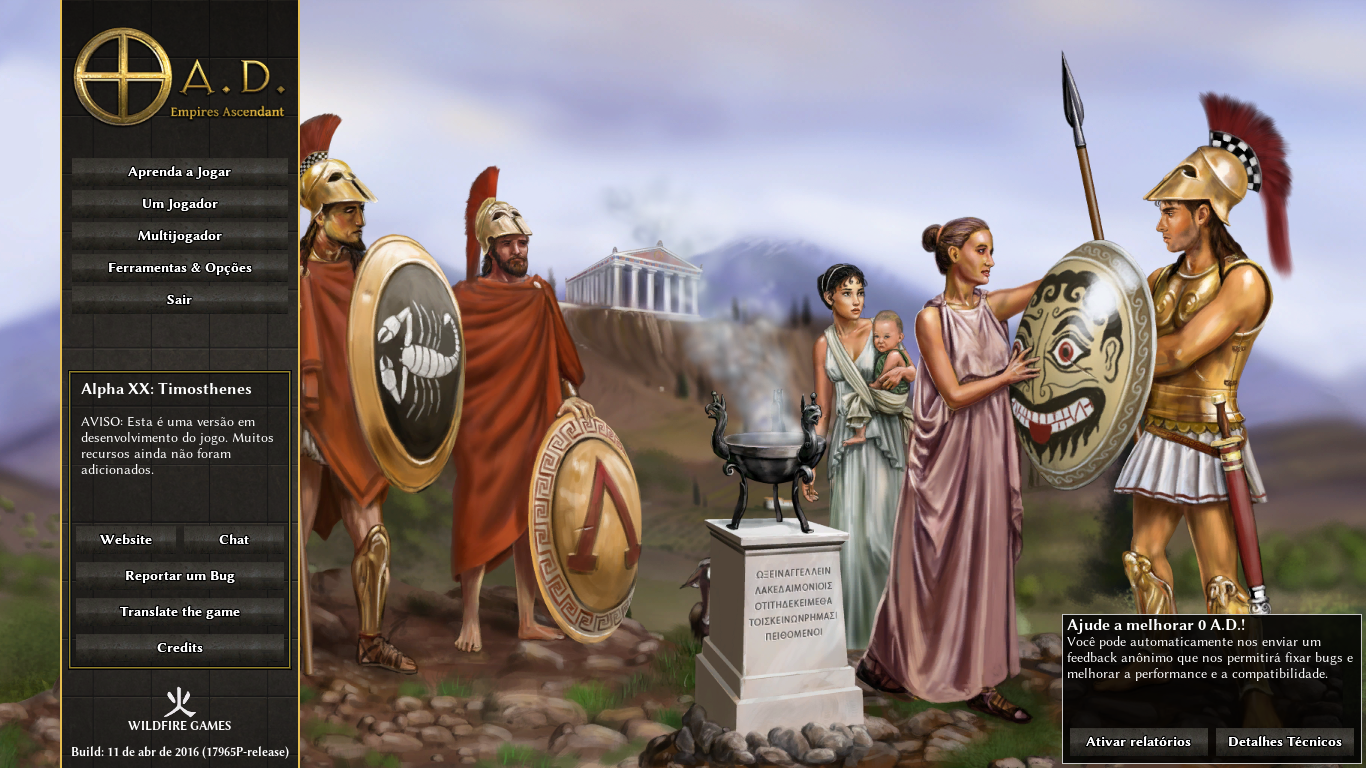
\includegraphics[width=0.9\linewidth]{screenshots_0ad/screenshot0006}
		\caption[]{Tela inicial do jogo 0A.D.}
		\label{fig:screenshot0006}
		
		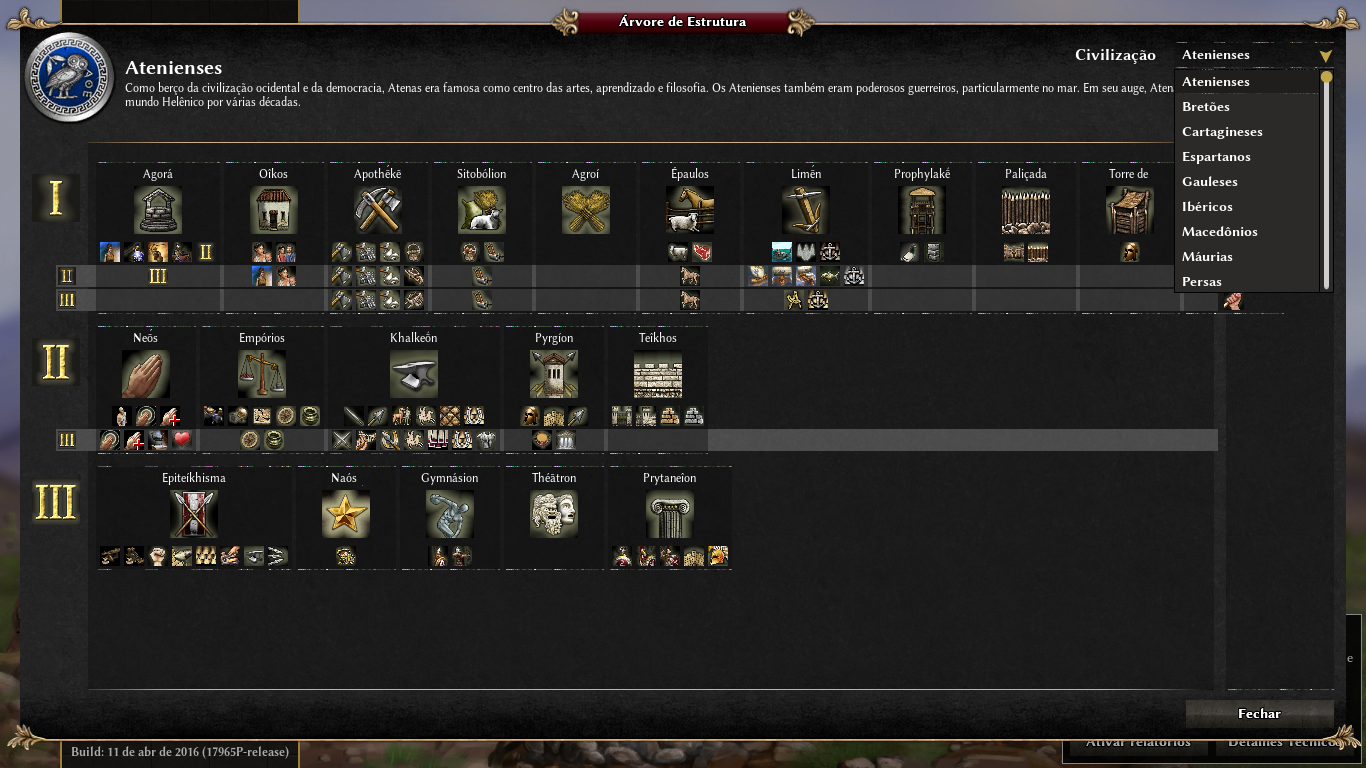
\includegraphics[width=0.9\linewidth]{screenshots_0ad/screenshot0007}
		\caption{Árvore de estrutura das civilizações retratadas no jogo}
		\label{fig:screenshot0007}
		
		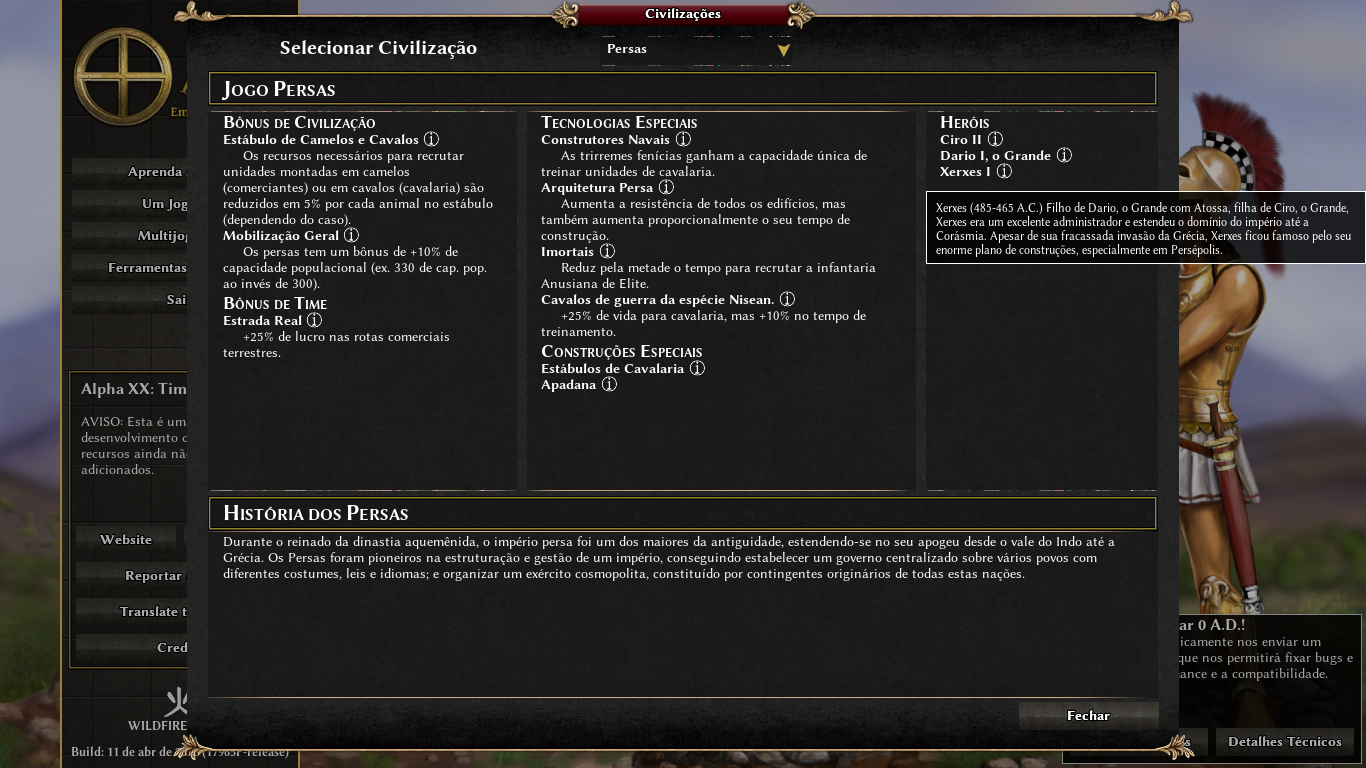
\includegraphics[width=0.9\linewidth]{screenshots_0ad/screenshot0008}
		\caption[]{Resumo da história, características e principais líderes de cada povo. No jogo é possível ter um desses líderes fazendo parte da população, ele é chamado de \textit{héroi}}
		\label{fig:screenshot0008}

	\end{figure}
	
		\begin{figure}
			\centering
			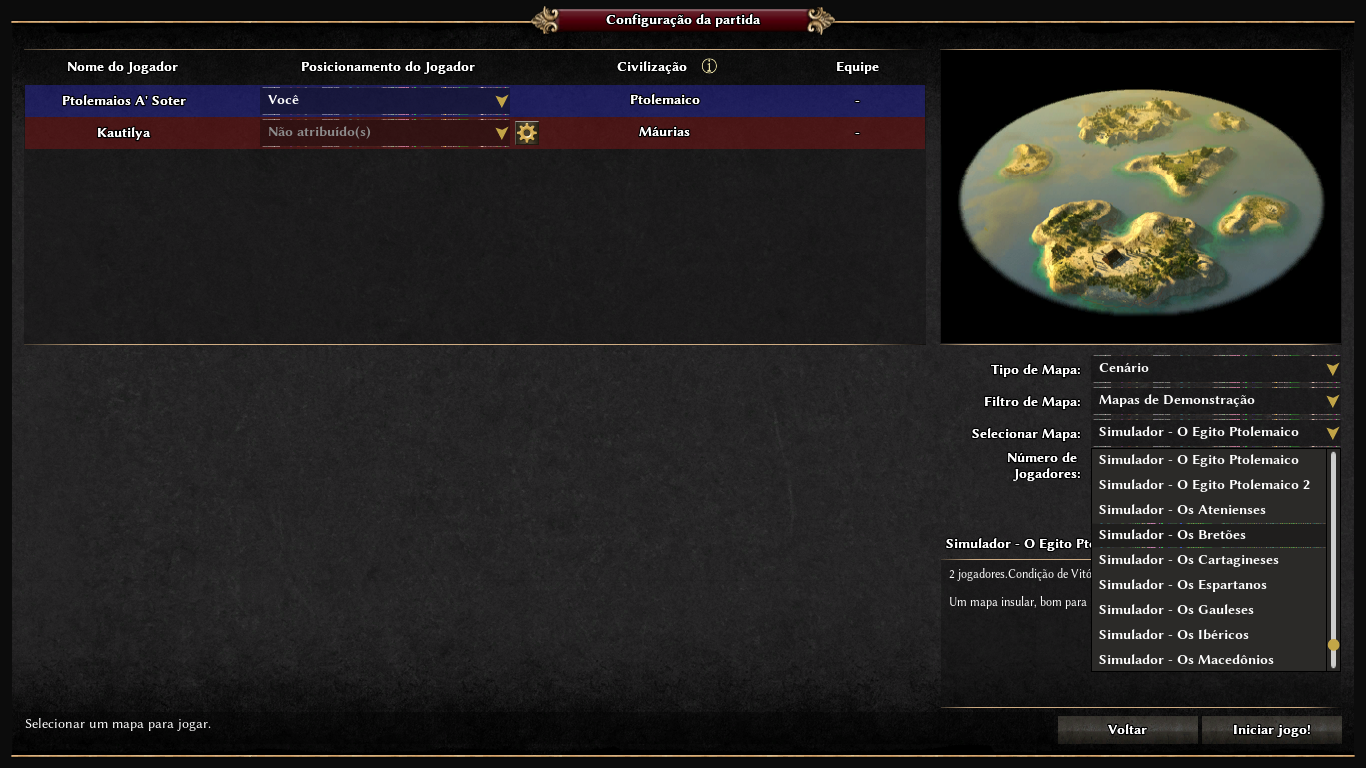
\includegraphics[width=0.9\linewidth]{screenshots_0ad/screenshot0009}
			\caption[]{Seleção de um mapa de demonstração que simule como era algum povo retratado no jogo}
			\label{fig:screenshot0009}
			
			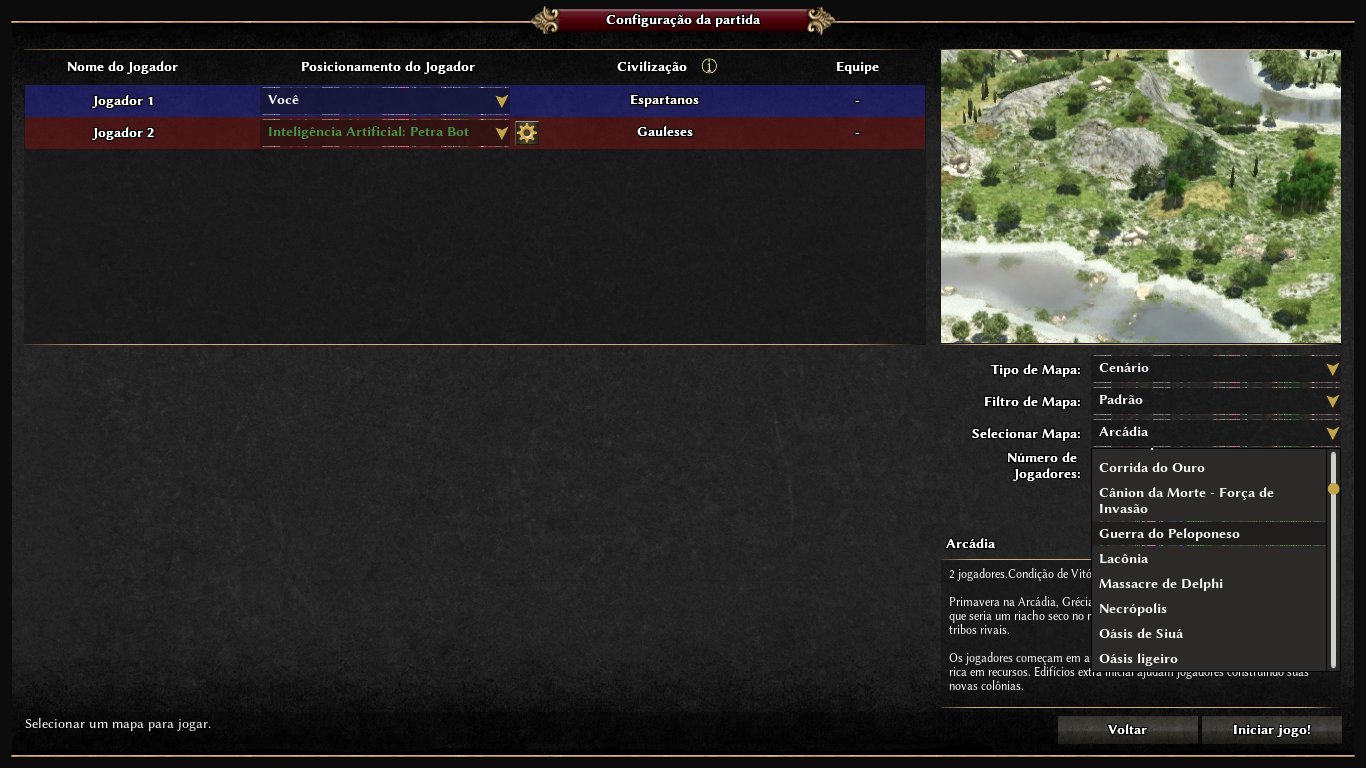
\includegraphics[width=0.9\linewidth]{screenshots_0ad/screenshot0010}
			\caption{No tipo de mapa \textit{cenário}, a seleção de níveis que representam batalhas históricas}
			\label{fig:screenshot0010}
			
			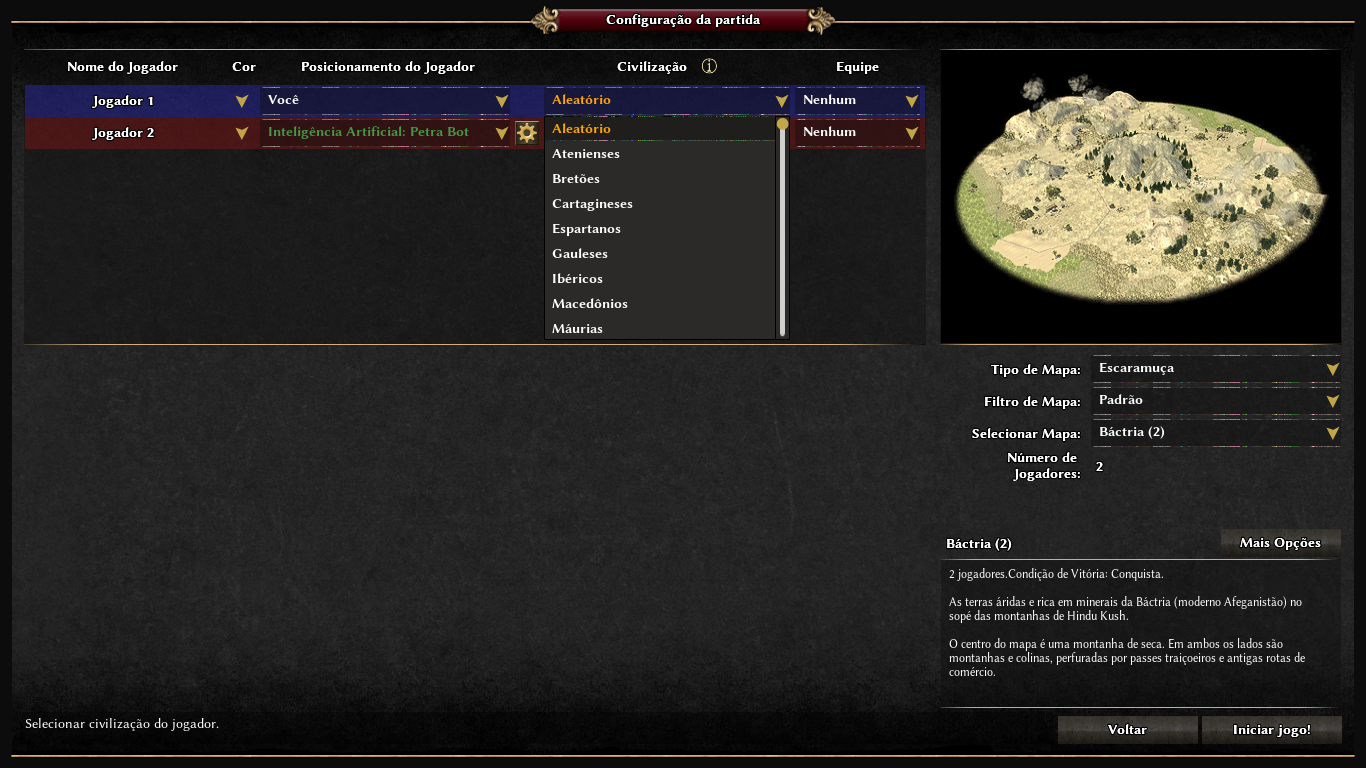
\includegraphics[width=0.9\linewidth]{screenshots_0ad/screenshot0011}
			\caption[]{No tipo de mapa \textit{escaramuça}, o jogador tem a liberdade de escolher o terreno e os povos}
			\label{fig:screenshot0011}
			
		\end{figure}

	\begin{figure}
		\centering
		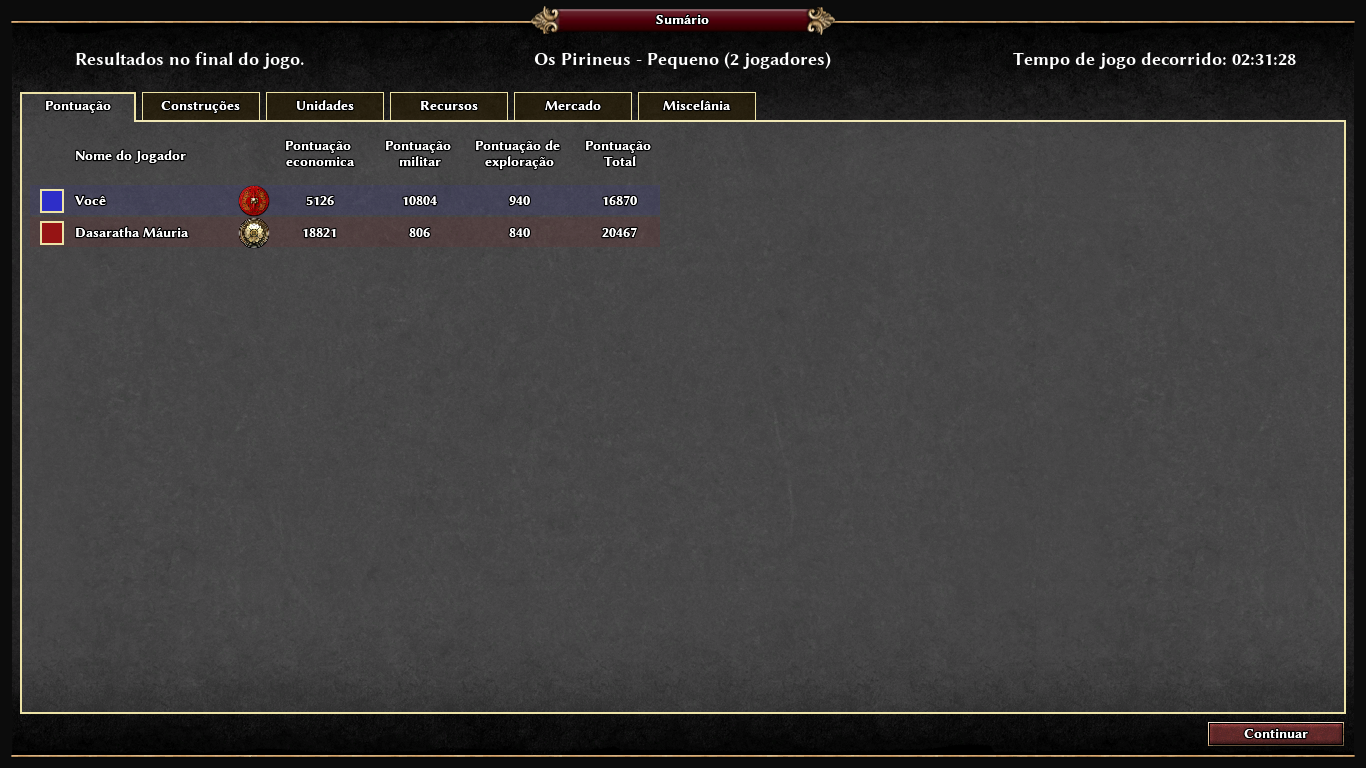
\includegraphics[width=0.9\linewidth]{screenshots_0ad/screenshot0012}
		\caption[]{Tela que mostra os dados ao final do jogo}
		\label{fig:screenshot0012}
		
		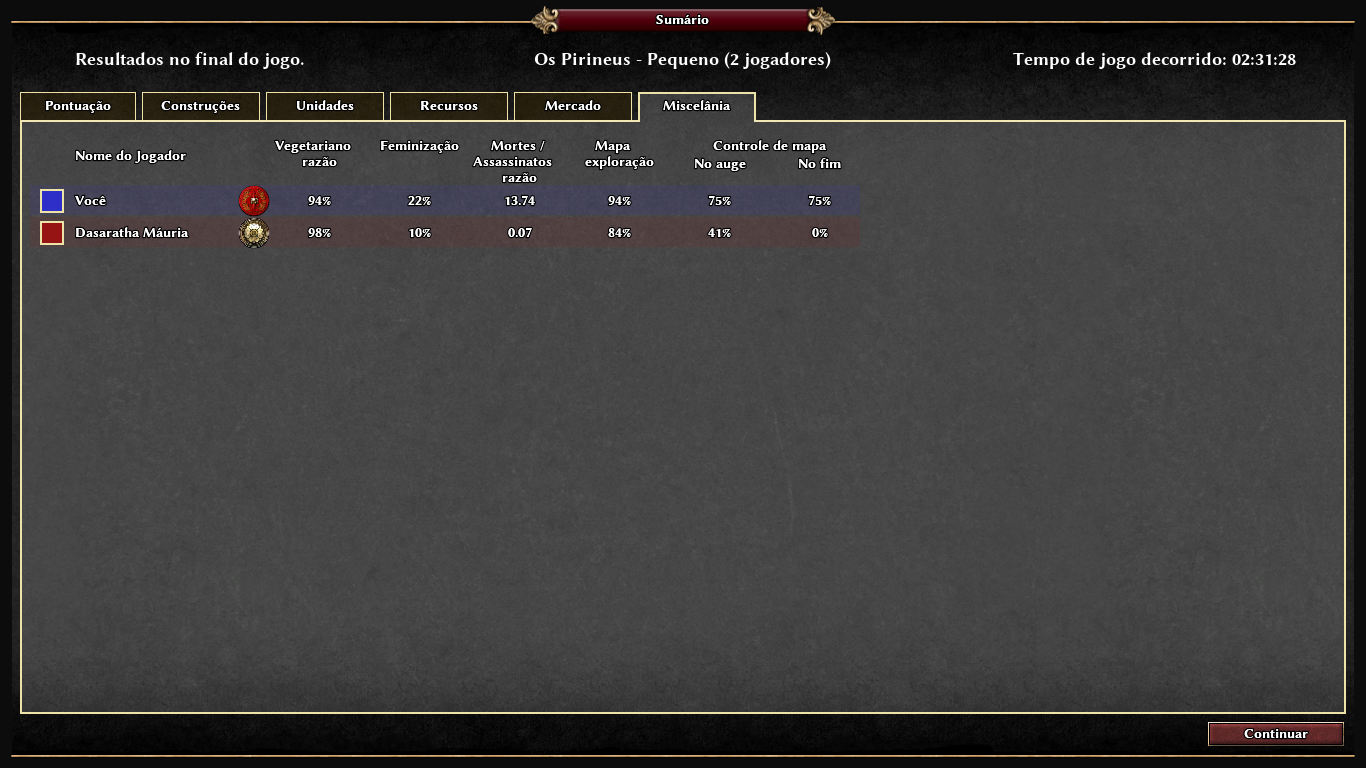
\includegraphics[width=0.9\linewidth]{screenshots_0ad/screenshot0013}
		\caption{Detalhe para a taxa de feminização}
		\label{fig:screenshot0013}
		
		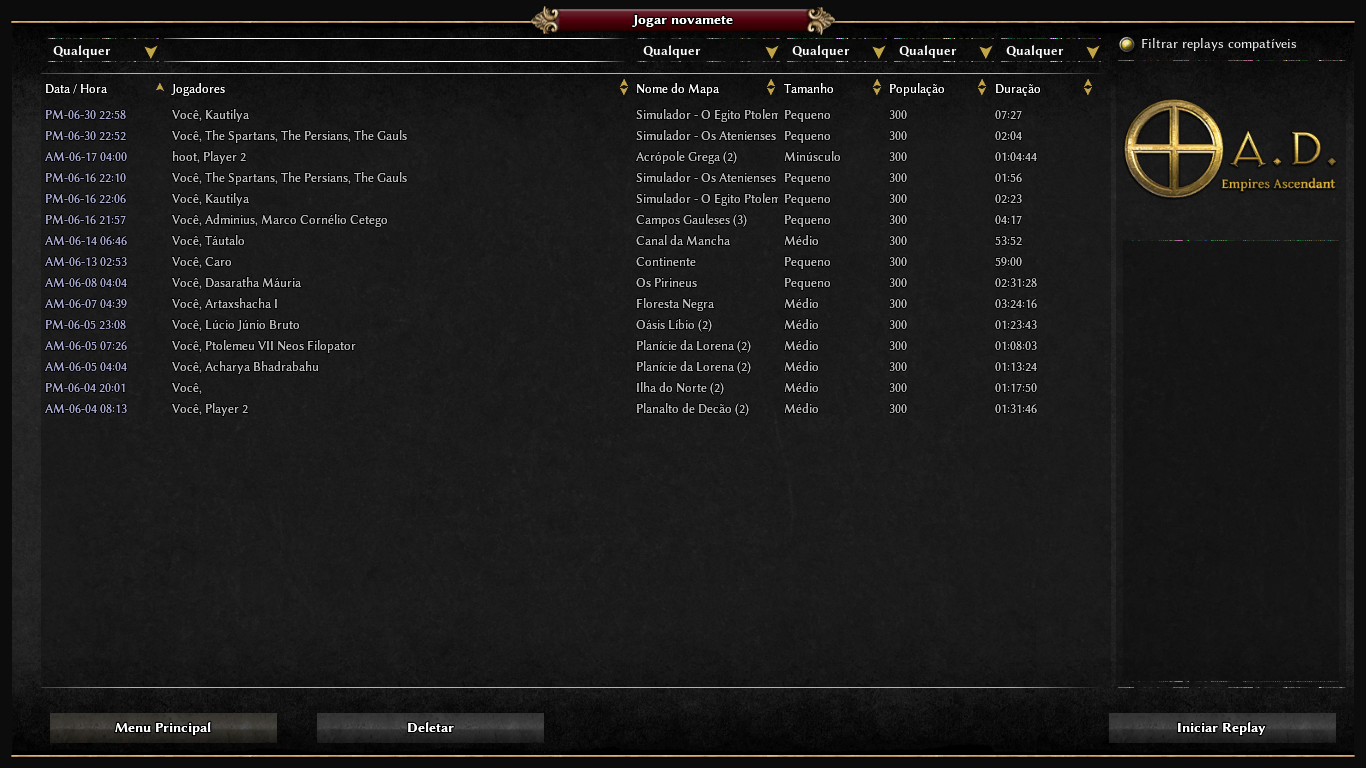
\includegraphics[width=0.9\linewidth]{screenshots_0ad/screenshot0014}
		\caption[]{Todas as partidas ficam salvas podendo ser vistas posteriormente quase como um vídeo interativo}
		\label{fig:screenshot0014}
		
	\end{figure}
	
	\begin{figure}
		\centering
		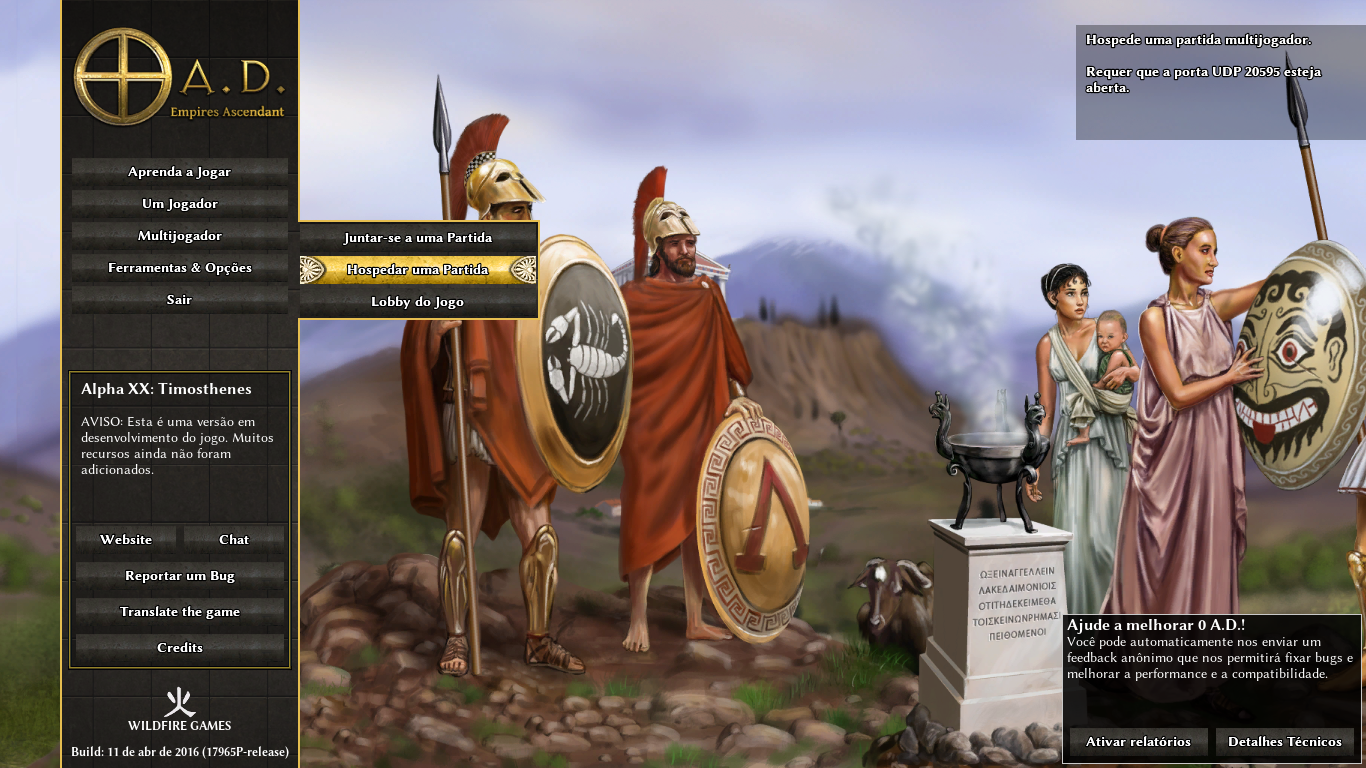
\includegraphics[width=0.9\linewidth]{screenshots_0ad/screenshot0015}
		\caption[]{Acesso a partida multiplayer e hospedagem de jogo}
		\label{fig:screenshot0015}
		
		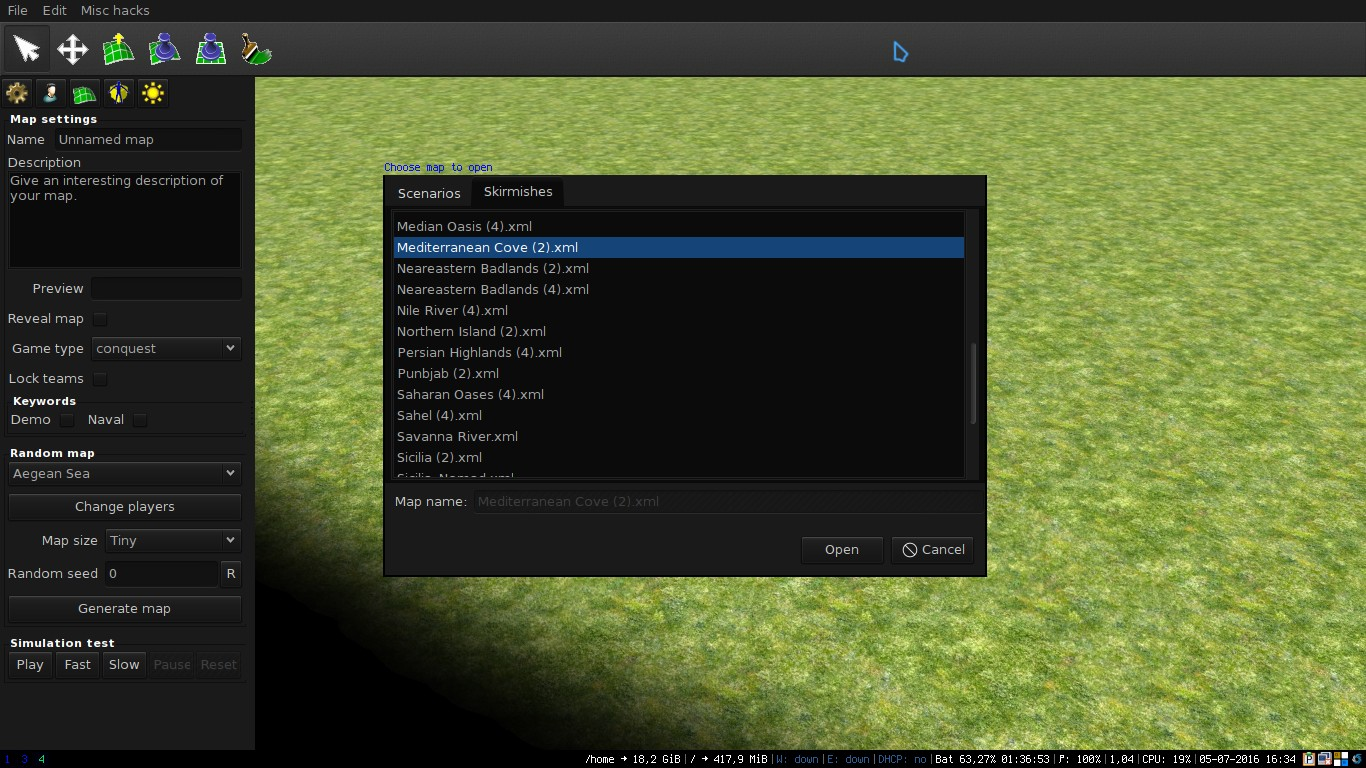
\includegraphics[width=0.9\linewidth]{screenshots_0ad/4_032.jpg}
		\caption{Editor de mapas (\texttt{Ferramentas -- Editor de cenário}) -- seleção de um mapa já pronto para ser modificado}
		\label{fig:4_032}
		
		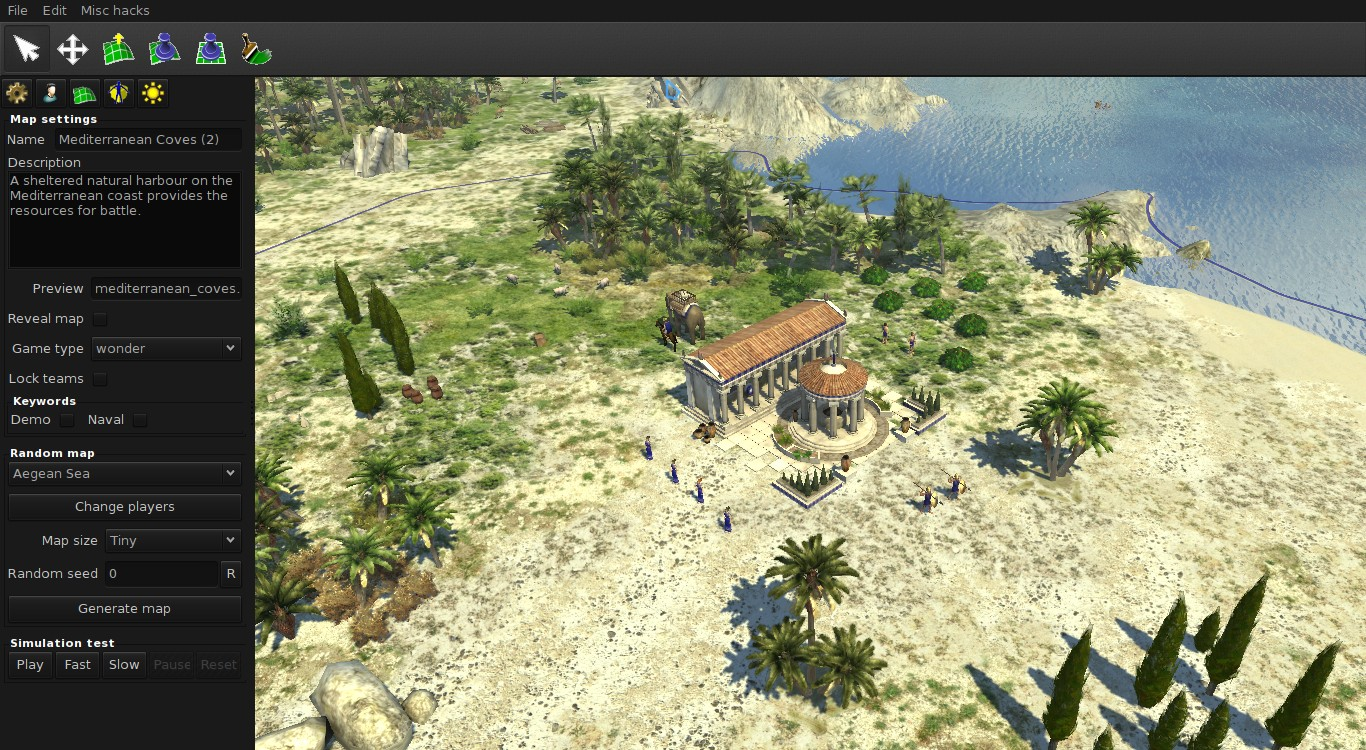
\includegraphics[width=0.9\linewidth]{screenshots_0ad/editor_de_cenario}
		\caption{Editor de mapas -- editando o mapa selecionado}
		\label{fig:4_03}
	
		
	\end{figure}

\end{document}
